% This is the Duke University Statistical Science LaTeX thesis template.
% It has been adapted from the Reed College LaTeX thesis template. The
% adaptation was done by Mine Cetinkaya-Rundel (MCR). Some of the comments
% that are specific to Reed College have been removed.
%
% Most of the work on the original Reed College document class and template
% was done by Sam Noble (SN). Later comments etc. by Ben Salzberg (BTS).
% Additional restructuring and APA support by Jess Youngberg (JY).
%
% See https://www.reed.edu/cis/help/latex/ for help. There are a
% great bunch of help pages there, with notes on
% getting started, bibtex, etc. Go there and read it if you're not
% already familiar with LaTeX.
%
% Any line that starts with a percent symbol is a comment.
% They won't show up in the document, and are useful for notes
% to yourself and explaining commands.
% Commenting also removes a line from the document;
% very handy for troubleshooting problems. -BTS

%%
%% Preamble
%%
% \documentclass{<something>} must begin each LaTeX document
\documentclass[12pt,twoside]{dukestatscithesis}
% Packages are extensions to the basic LaTeX functions. Whatever you
% want to typeset, there is probably a package out there for it.
% Chemistry (chemtex), screenplays, you name it.
% Check out CTAN to see: http://www.ctan.org/
%%
\usepackage{graphicx,latexsym}
\usepackage{amsmath}
\usepackage{amssymb,amsthm}
\usepackage{longtable,booktabs,setspace}
\usepackage{chemarr} %% Useful for one reaction arrow, useless if you're not a chem major
\usepackage[hyphens]{url}
% Added by CII
\usepackage{hyperref}
\usepackage{lmodern}
\usepackage{float}
\floatplacement{figure}{H}
% End of CII addition
\usepackage{rotating}

% Next line commented out by CII
%%% \usepackage{natbib}
% Comment out the natbib line above and uncomment the following two lines to use the new
% biblatex-chicago style, for Chicago A. Also make some changes at the end where the
% bibliography is included.
%\usepackage{biblatex-chicago}
%\bibliography{thesis}


% Added by CII (Thanks, Hadley!)
% Use ref for internal links
\renewcommand{\hyperref}[2][???]{\autoref{#1}}
\def\chapterautorefname{Chapter}
\def\sectionautorefname{Section}
\def\subsectionautorefname{Subsection}
% End of CII addition

% Added by CII
\usepackage{caption}
\captionsetup{width=5in}
% End of CII addition

% \usepackage{times} % other fonts are available like times, bookman, charter, palatino


% To pass between YAML and LaTeX the dollar signs are added by CII
\title{Modelling Altcoin Price Variation with Sentiment Based Predictors}
\author{Daniel Spottiswood}
% The month and year that you submit your FINAL draft TO THE LIBRARY (May or December)
\date{May 2020}
\advisor{Sayan Mukherjee}
\institution{Duke University}
\degree{Bachelor of Science in Statistical Science}
\committeememberone{Amy Herring}
\committeemembertwo{Fan Li}
\dus{Dus X. Name}
%If you have two advisors for some reason, you can use the following
% Uncommented out by CII
% End of CII addition

%%% Remember to use the correct department!
\department{Department of Statistical Science}

% Added by CII
%%% Copied from knitr
%% maxwidth is the original width if it's less than linewidth
%% otherwise use linewidth (to make sure the graphics do not exceed the margin)
\makeatletter
\def\maxwidth{ %
  \ifdim\Gin@nat@width>\linewidth
    \linewidth
  \else
    \Gin@nat@width
  \fi
}
\makeatother

\renewcommand{\contentsname}{Table of Contents}
% End of CII addition

\setlength{\parskip}{0pt}

% Added by CII

\providecommand{\tightlist}{%
  \setlength{\itemsep}{0pt}\setlength{\parskip}{0pt}}

\Acknowledgements{
I want to thank a few people.
}

\Dedication{
You can have a dedication here if you wish.
}

\Preface{
This is an example of a thesis setup to use the reed thesis document
class (for LaTeX) and the R bookdown package, in general.
}

\Abstract{
This is a placeholder
}

% End of CII addition
%%
%% End Preamble
%%
%
\begin{document}

% Everything below added by CII
  \maketitle

\frontmatter % this stuff will be roman-numbered
\pagestyle{empty} % this removes page numbers from the frontmatter
  \begin{acknowledgements}
    I want to thank a few people.
  \end{acknowledgements}
  \begin{preface}
    This is an example of a thesis setup to use the reed thesis document
    class (for LaTeX) and the R bookdown package, in general.
  \end{preface}
  \hypersetup{linkcolor=black}
  \setcounter{tocdepth}{2}
  \tableofcontents

  \listoftables

  \listoffigures
  \begin{abstract}
    This is a placeholder
  \end{abstract}
  \begin{dedication}
    You can have a dedication here if you wish.
  \end{dedication}
\mainmatter % here the regular arabic numbering starts
\pagestyle{fancyplain} % turns page numbering back on

This is a placeholder for the abstract.

\chapter*{Introduction}\label{introduction}
\addcontentsline{toc}{chapter}{Introduction}

Since Bitcoin's introduction in 2008, Blockchain has been touted as a
revolutionary technology capable of rapidly modernizing the entire
financial system in part by enabling the spread of cryptocurrencies.
While these lofty goals have yet to be realized, the rapid ascension of
Bitcoin and many other cryptocurrencies have made many extremely
wealthy. Hobbyist investors hoping to replicate these same fortunes,
have flocked to cryptocurrencies in search of high volatility investment
vehicles with significant upside.

It is not a stretch to claim that these marketplaces have displayed many
characteristics more synonymous with gambling than other regulated
financial products. Market manipulation, specifically pump and dump
schemes are rampant and relatively unchecked with Reddit and other
forums dictating large market movements(Tao Li, Shin, \& Wang, 2019). A
recent study also found strong correlations between cryptocurrency
trading and both high risk stock trading and gambling, the latter of
which has been shown to succumb to human biases(Mills \& Nower, 2019,
Vernon (2003)).

A core feature of cryptocurrency markets is the lack of easily
calculable intrinsic value in the underlying products. The value of a
cryptocurreny is largely determined by its popularity and usage, leading
to a feedback loop as value and popularity build upon each other.
Without clear bounds of reasonable valuations, these currencies make
large swings often with no underlying changes in the core products or
macroeconomic landscape. For the statistically inclined, this has
provided an interesting opportunity to attempt to model these seemingly
random fluctuations in both price and sentiment. JP Koning describes the
problem as attempting to ``anticipate what average opinion expects
average opinion to be'', no simple task(2019).

While sentiment indicators have been used to predict equities for
decades, they seem particularly applicable in the prediction of
cryptocurrencies due to their derivation of value. Researchers have
shown that forum comments, Wikipedia and Google search volumes, and
Twitter comments can be utilized to predict a variety of
cryptocurrencies with varying levels of accuracy(Kristoufek, 2013,Tianyu
Li, Chamrajnagar, Fong, Rizik, \& Fu (2019), Y. Kim et al. (2001)). Long
short term memory (LSTM) neural nets, extreme gradient boosted trees
(XGBoost), and vector autoregression have been shown to have success in
this context.

However, much of the academic research in this space has focused on
Bitcoin and the use of a single class of predictors. Many researchers
have either shown correlations between predictions and prices or success
in binary prediction, but have failed to propose profitable strategies
that consistently outperform the market(Tianyu Li et al., 2019,
Colianni, Rosales, \& Signorotti (2015)).

In this paper, I predict price movements in altcoin, Zcash. Zcash
originated as a fork from the Bitcoin blockchain in 2016 albeit with a
different name: Zerocoin protocol. Zcash provides the option for users
to shield their identities and amount during a transaction, through
zero-knowledge cryptography. Although it has gained recognition through
its privacy features, as of May 2018 less than one percent of
transactions were fully shielded, supporting the thesis that those
trading Zcash are apathetic towards the specifics of the
technology(Floyd, 2018). I chose Zcash, ticker ZEC, because it has
moderately high volume, twenty-second in market capitalization among
cryptocurrencies, has stable but developing technology, and has a unique
and distinguishable name/ticker.

I use search volume, buy/sell volume, and twitter text sentiment
combined with XGBoost and LSTM Neural nets to predict hourly price
movements in Zcash. I propose strategies that are shown, through the use
of walk-forward testing, to return over 200 percent net fees in a span
of approximately one hundred days. My approach adds to the current state
of academic research by utilizing this combination of features to
propose strategies that return substantial profits in an altcoin market.
Furthermore, these strategies and models operate at the hourly level,
whereas previous research has focused on daily returns.

In Section \ref{data}, I use advanced methods to estimate tweet
sentiment based on hourly data with tweets from suspected bots removed.
I normalize Google search volume for Zcash by benchmarking it to the
search volume of the largest cryptocurrency, Bitcoin. In section
\ref{method}, I detail the XGBoost and LSTM models I use as well as my
decision to regress on log returns. In section \ref{results} I use
walk-forward testing to estimate the theoretical profits of trading
strategies based on these predictions. I dig into the models in an
attempt to parse out how sentiment and volume may interact to drive
price movements in certain situations.

In conclusion, I discuss what these results may demonstrate regarding
market dynamics. I also examine the feasibility of implementation given
the current exchange landscape, including liquidity and fees.

\chapter*{Literature Review}\label{literature-review}
\addcontentsline{toc}{chapter}{Literature Review}

Early work demonstrated the predictive power of twitter sentiment on
large-cap stocks(Tushar \& Srivastava, 2012). Oliveira et al. used a
Kalman filter to combine twitter sentiment with longer-term popular
survey sentiment indicators(2017).

Recently this research has been extended into cryptocurrency, arguably a
much better application, with academics demonstrating the predictive
power of Twitter sentiment and Wikipedia and Google search volume on
cryptocurrency prices. Garcia and Schweitzer provided proof of concept
using Twitter sentiment and volume to predict Bitcoin prices(2015). They
made additional use of technical market features and applied a
multi-dimensional model of vector autoregression to achieve a Sharpe
ratio of 1.77. They found that higher polarization was correlated with
rises in Bitcoin.

Tianyu Li et al. demonstrated the effectiveness of Twitter sentiment in
predicting the altcoin, Zclassic(Tianyu Li et al., 2019). They
determined that 3 hours was the timeframe over which sentiment is fully
absorbed into the price, and after extensive cross-validation, they had
the most success using extreme gradient boosting. They made use of an
additional feature that more heavily weighted retweets due to their
network effect.

Kim et al. displayed a similar effect with user comments on relevant
cryptocurrency online communities, displaying predictive power on both
price and volume for several of the largest cryptocurrencies(2001). They
utilized sets of keywords to determine relatedness to certain concepts
in addition to the direction of sentiment.

ElBahrawy et al. displayed significant theoretical returns on a
Wikipedia based trading strategy(2019). Kristoufek paired the Wikipedia
data with Google trends to develop a multi-feature trading strategy
using vector autoregression and vector error-correction(2013). He
demonstrated that when prices are high increased interest tends to push
prices higher, and vice-versa. This behavior may explain both the high
volatility and frequencies of bubbles in the crypto space. This work was
continued by Alexander Dickerson who used a set of Wikipedia and Google
search frequencies to build trading strategies(2018). While they appear
to be extremely profitable due to testing throughout the bitcoin boom
they are not able to adequately predict the subsequent crash. As the
cryptocurrency space has experienced many long term swings, it is
important that these algorithms are robust enough to remain accurate in
the event of novel changes in the dynamics of the market. This is an
issue across much of the research in this space as studies often have
too small a scope to measure realistic applicability or they predict
across the entirety of the cryptocurrency era in which prices, for the
most part, have consistently risen. The latter allows models to overfit
and display high theoretical profitability.

Outside of the sentiment/social information space, Wei demonstrated
success using solely technical market information and an LSTM neural
net(2018). Using a sliding window transformation, he exhibited profits
while trading on a daily timescale producing an F1 score of almost 60\%
when making binary predictions.

It is important to note that while all of this proof of concept research
has demonstrated significant profits, few have taken into account
transaction fees or the price of liquidity. It is unclear whether these
strategies would be profitable if implemented in the real world,
although many show high enough returns to infer profitability. The
combination of transaction fees and spreads can be in the range of 20 to
100 basis points, therefore profitable strategies require a significant
edge per trade. In practice, various tactics can be used to reduce
transaction costs of different strategies, but the impact of these
tactics will vary by strategy.

\chapter{Data}\label{data}

Data was collected in weekly increments from October 20th to March 17th,
accumulating in over 3,500 data points.

\section{Twitter}\label{twitter}

Twitter is one of the largest social media platforms, distinct in its
focus on brief text. It has a large cryptocurrency community with a
combination of individual traders and key moguls who dictate the trading
flow of thousands of followers.

The Twitter API allows one to pull all tweets containing certain
keywords. I collected all tweets in English containing the terms `zcash'
or `zec'. With over 130 thousand relevant tweets during the specified
time period, there are on average 37.5 tweets every hour before
accounting for bots or other confounding factors.

To remain consistent with the other features, I aggregated the Twitter
data by the hour. As shown in Figure \ref{fig:dailytweets}, while there
is a daily trend in the number of tweets every hour the autocorrelation
is not extreme enough to require adjustment. I chose to explore the mean
sentiment, a favorite weighted sentiment, and a retweet weighted
sentiment as well as the tweet count. Testing showed that the mean
sentiment, retweet weighted sentiment, and tweet count, were
instrumental to the model, while the favorite weighted sentiment seemed
to add noise and caused the model to overfit.
\begin{figure}
\centering
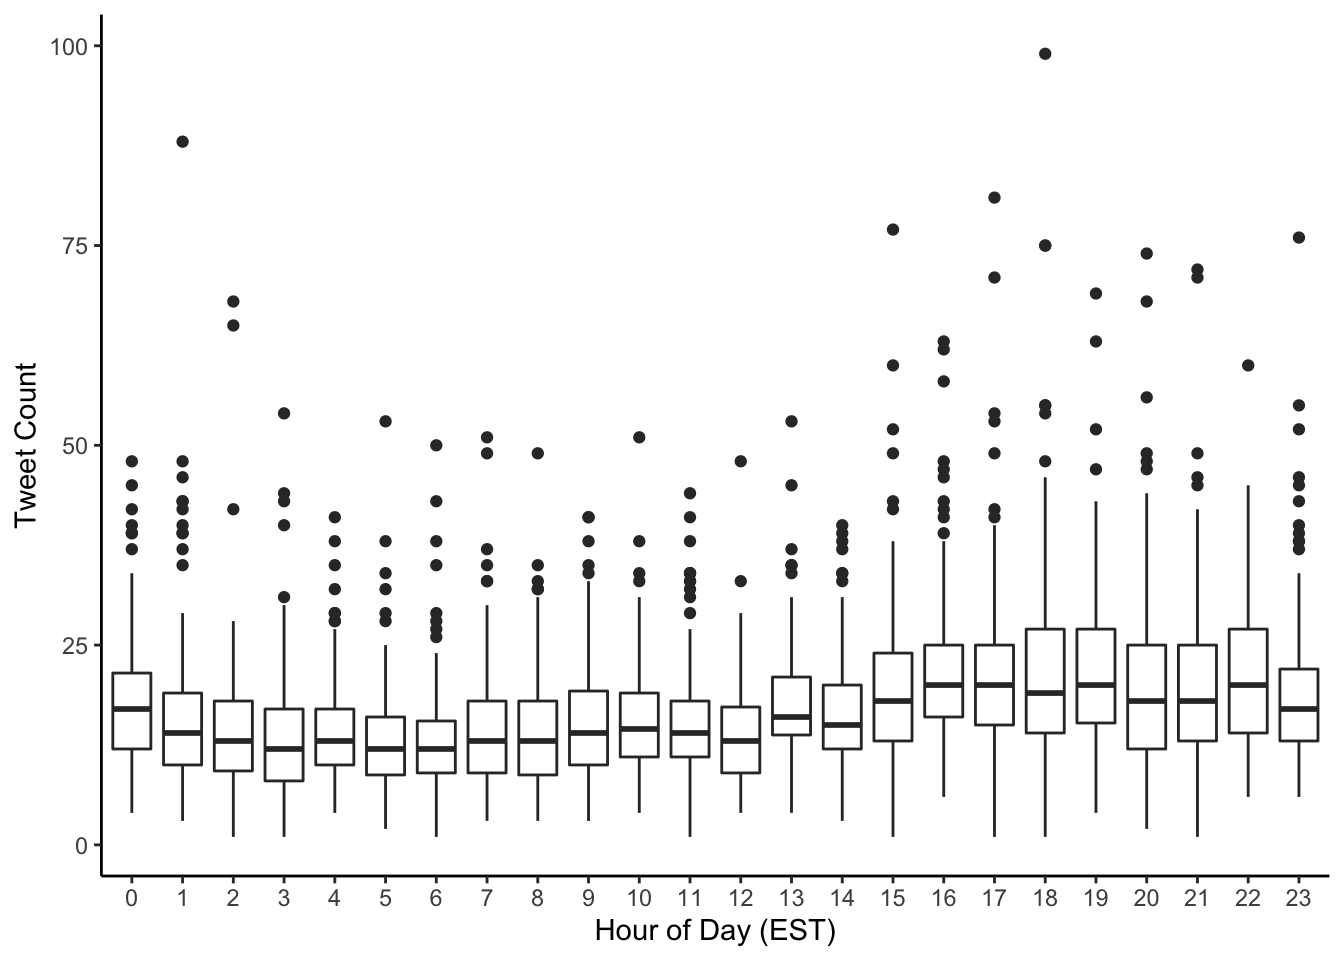
\includegraphics{thesis_files/figure-latex/dailytweets-1.pdf}
\caption{\label{fig:dailytweets}Hourly Tweet Counts}
\end{figure}
\subsection{Tweet Removal}\label{tweet-removal}

While I previously described the unique name as being one of the
deciding factors in choosing Zcash, a hurdle arose as the string `zec'
appears both in Zechariah, a Hebrew prophet, and is an acronym for the
Zimbabwe Electoral Commission. A nonnegligible portion of the tweets
collected, approximately 2-3\%, referenced one of these two topics.
Therefore, I removed all tweets containing `Zechariah' as well as common
terms appearing in relation to the election: `election', `Zimbabwe',
`Botswana', etc..

Twitter has taken aggressive measures to remove bots from its platform.
However, a recent study estimated that 9 to 15\% of accounts are bots
while another study found that two-thirds of shared links are posted by
bots(Wojcik, n.d.,Varol, Ferrara, Davis, Menczer, \& Flammini (2017)).
This may be even higher in the cryptocurrency space due to the potential
profits if one can swing public opinion. I use Michael Kearney's
`tweetbotornot' package to eliminate this noise by classifying and
removing bots. Michael Kearney's package applies an extreme gradient
boosting model to a user's tweets and bio to predict whether or not they
are a bot with over 93\% accuracy. Due to the high number of bots and
the large number of tweets that they post, I do not expect these
accuracy rates to transfer perfectly onto my dataset. I manually tested
30 users that were classified as bots and 30 users classified as
non-bots, the results are shown in Table \ref{tab:botexp}. An unknown
refers to an account that was removed, which we can speculate would
often be bots. This test used a .7 threshold that was selected in the
validation phase. My own distinctions are not objective, so blind
testing was performed to eliminate partial bias from these results. The
results show statistically significant differences between the groups.
Out of the 15 bots, most were classified correctly, however there was
still a significant portion of false positives. While this is
concerning, it seems likely that for modeling purposes it is more
important to remove the systematic bias of bots than to capture the full
extent of the authentic signal. This was supported empirically as it was
advantageous to remove a larger portion of bots at the expense of
removing some authentic accounts.

\label{tab:botexp}Bot Model Accuracy

True

False

Unknown

Bot

14

4

12

Non-Bot

26

1

3

Overall slightly over half of the users and half of the tweets were
removed. After removing tweets not related to the cryptocurrency Zcash
and those posted by potential bots, the dataset contains approximately
57 thousand tweets for an average of 16 tweets per hour.

\subsection{Sentiment Analysis}\label{sentiment-analysis}

R has multiple packages that perform sentiment analysis on texts. I
implemented two of the most popular libraries The `SentimentAnalysis'
package allows the use of many different dictionaries, however, I chose
the two most suitable to my goals: Henry's finance specific dictionary
and the QDAP dictionary put together by Tyler Rinker. `SentimentR'
similarly utilizes the QDAP dictionary, however it also takes into
account valence shifters such as negators to improve performance over a
simple dictionary lookup while still maintaining speed. To assess
performance, I randomly sampled 100 tweets and cross-checked their
predictions using my own classifications as the ground truth. The
results are shown in Table \ref{tab:sentimentexp}. Tweets were
classified into three groups: positive, neutral, and negative.
`Sentimentr' had the best performance when looking at weighted F1
scores, which given the class imbalance is a better measurement of
accuracy.
\begin{align}
  Weighted \; F1 = \sum_{i=1}^{numclasses}{2*\frac{(precision_{class_i} + recall_{class_i})}{(precision_{class_i}*recall_{class_i})}} \label{eq:1} \\ 
\end{align}
\label{tab:sentimentexp}Sentiment Package Accuracy

Henry's Financial

QDAP

SentimentR

F1

0.55

0.62

0.62

Weighted F1

0.62

0.63

0.70

The confusion matrix using `SentimentR' is in Table
\ref{tab:sentimentcheck}. It is important to note that most of the
errors occur through neutral samples being labeled as positive or
negative and vice-versa. There are relatively few occurrences of
negative/positive samples being classified as the opposite. One example
of a negative outlook tweet that was labeled as positive is the
following: ``All privacy coins are held together with duct tape +
paperclips, in particular, all XMR and ZEC forks. Epic work
by\ldots{}''. This is a tweet that even the most sophisticated NLP
algorithm would struggle with due to the ambiguity of the metaphor and
the positive connotation of ``epic''.

\label{tab:sentimentcheck}SentimentR Confusion Matrix

Obs. Negative

Obs. Neutral

Obs. Positive

Negative

6

8

9

Neutral

0

26

8

Positive

3

14

26

\section{Google Search Volume}\label{google-search-volume}

Google trends display normalized search volume for a given keyword. I
collected trends data for the terms `zec', `zcash', and `bitcoin'. I use
the ratio of `zec' and `zcash' search volumes to `bitcoin' in order to
normalize for general trends in the interest in cryptocurrency and also
included the raw `zcash' value. Figure \ref{fig:dailygtrends}
illustrates that the hourly ratios do not display autocorrelation to an
extent that requires correction.
\begin{figure}
\centering
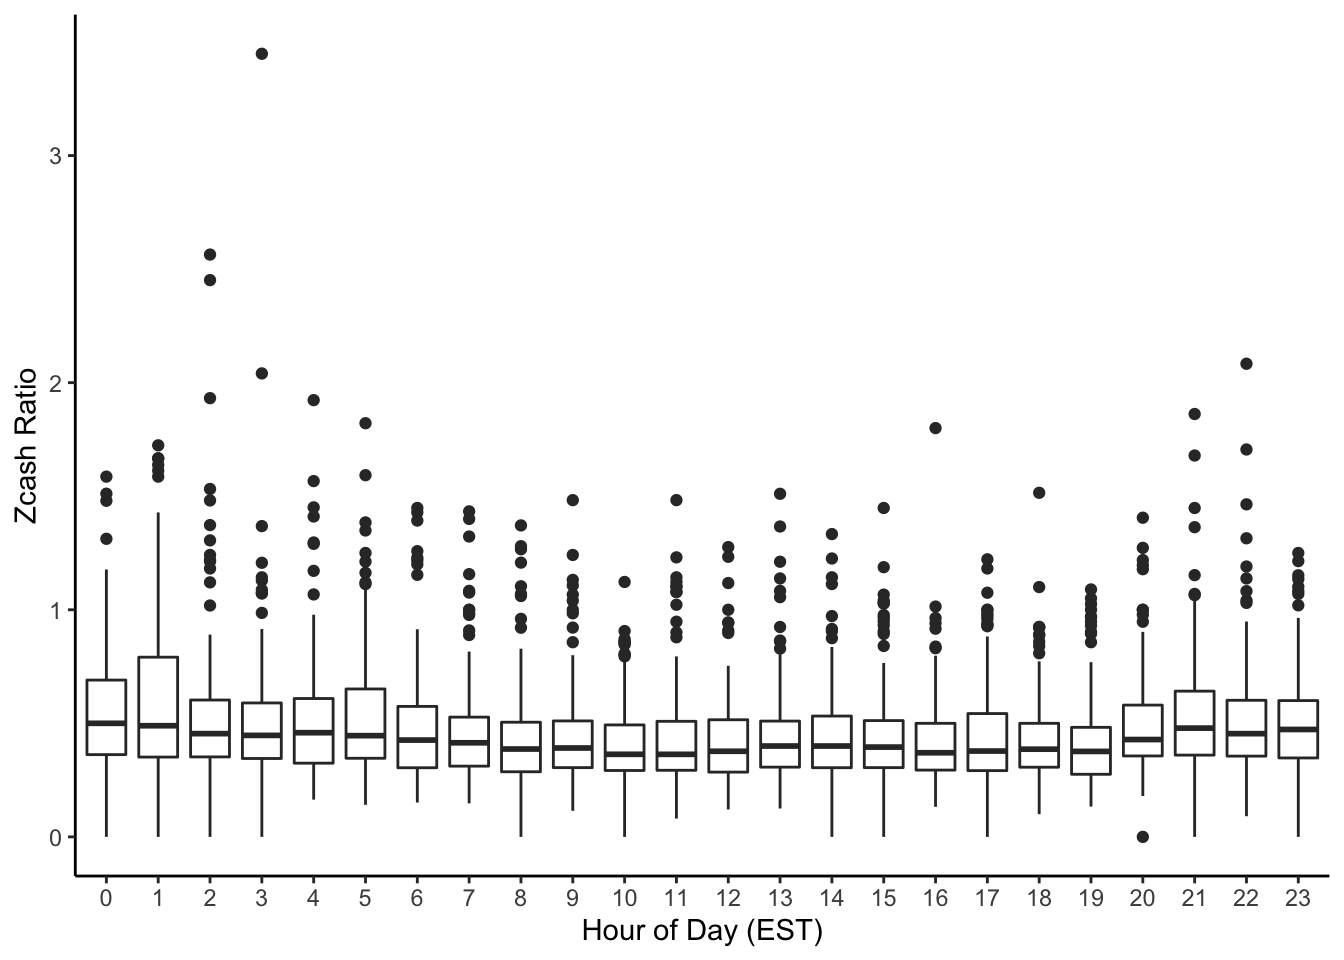
\includegraphics{thesis_files/figure-latex/dailygtrends-1.pdf}
\caption{\label{fig:dailygtrends}Hourly Gtrends ratios}
\end{figure}
\section{Price and Volume}\label{price-and-volume}

Cryptocompare uses a sophisticated aggregation method to accurately
assess real prices for cryptocurrencies given the multitude of markets
with different liquidity and regulations. They use a volume-weighted
average with an additional decay based on the time since the most recent
trade and outlier detection.

Volume to and volume from correspond to the volume in and out of a
certain currency in the pair. I use the conversion rate of ZEC to USD.
Interestingly as shown in \ref{fig:}, as price increased in January and
early February the volume initially increased dramatically, but then
tailed off.
\begin{figure}
\centering
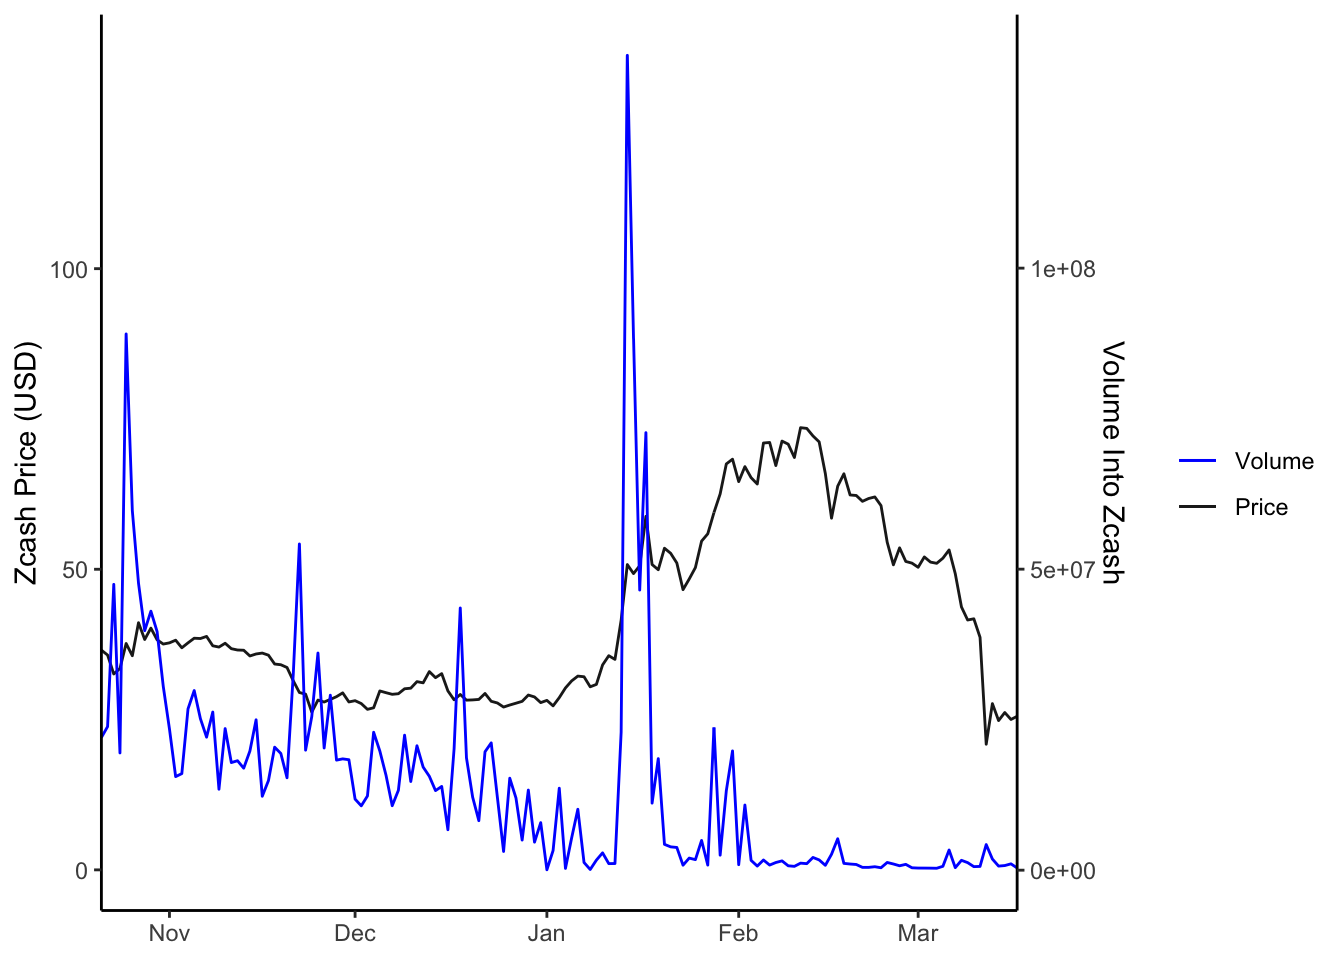
\includegraphics{thesis_files/figure-latex/unnamed-chunk-2-1.pdf}
\caption{}
\end{figure}
\section{Exploratory Data Analysis}\label{exploratory-data-analysis}

Correlations between the model features and four hour log returns are
shown in Figure \ref{fig:correlations}.
\begin{figure}
\centering
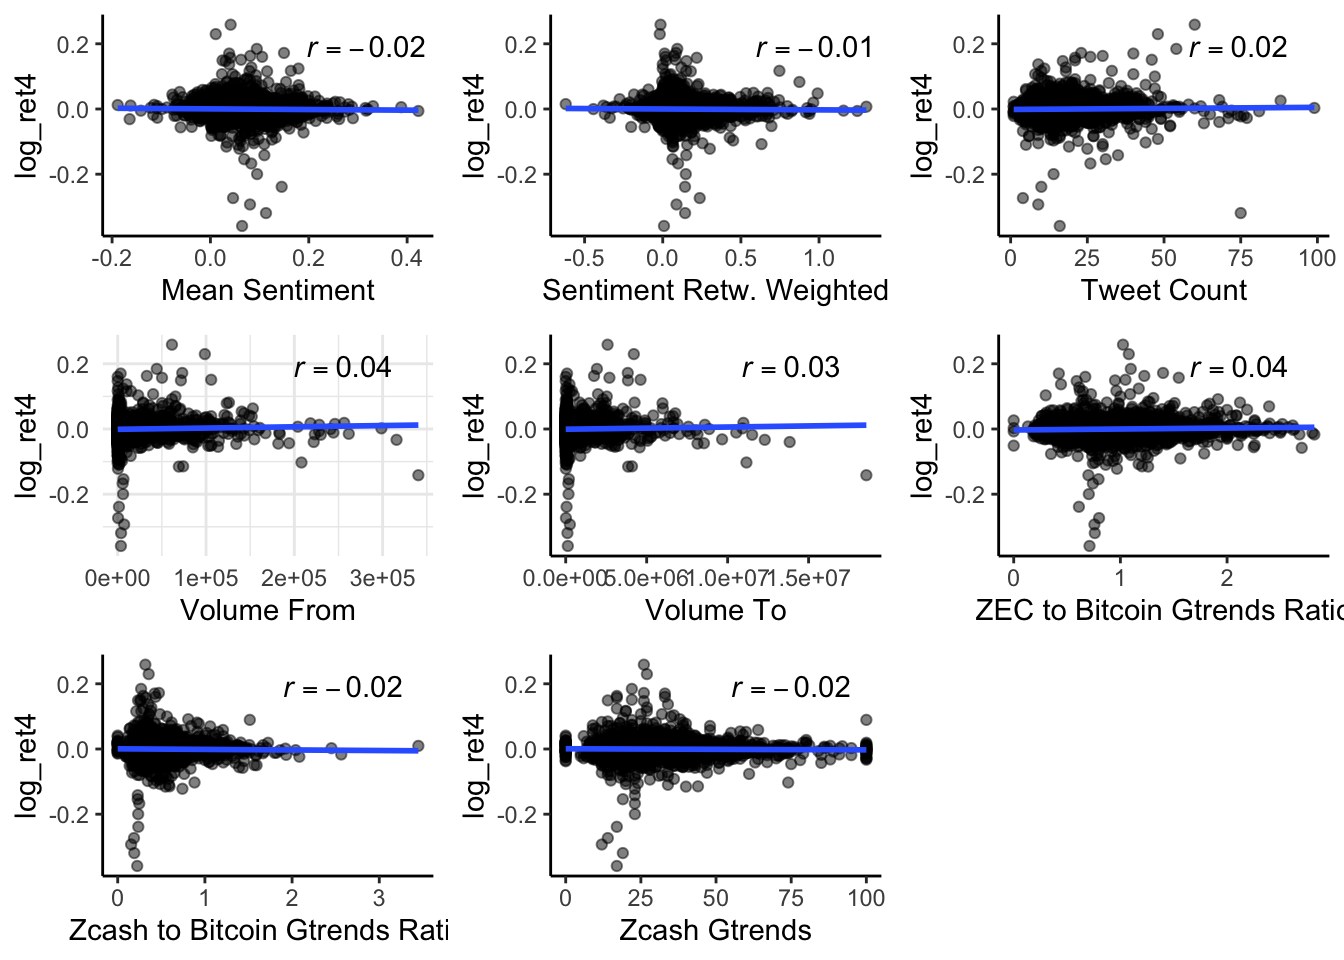
\includegraphics{thesis_files/figure-latex/correlations-1.pdf}
\caption{\label{fig:correlations}Correlations with Log Returns}
\end{figure}
\chapter{Methodology}\label{method}

\section{Log Returns}\label{log-returns}

I regress on log returns with a specified lag of 4 hours that was
determined in the validation phase. This is not necessarily equivalent
to the time it takes for the full effect of the sentiment to be
realized, but may be an optimization of the tradeoff between signal and
noise.
\begin{align}
  log \:  return_i = log(\frac{p_{(i)}}{p_{(i-lag)}}) \label{eq:5} \\ 
\end{align}
This provides multiple advantages over price or raw returns (``Why log
returns,'' 2012).
\begin{enumerate}
\def\labelenumi{\arabic{enumi}.}
\tightlist
\item
  Under the assumption that prices follow a log normal distribution than
  log returns are normally distributed
\item
  When returns are small log-returns are close in value
\item
  Compound returns are normally distributed as the sum of normally
  distributed log returns
\end{enumerate}
The distribution of log returns for Zcash is shown in Figure
\ref{fig:logrets}. It should be noted that log returns do not fully
adhere to a normal distribution due to the frequent multiple standard
deviation occurences\footnote{For QQPlot see appendix}.
\begin{figure}
\centering
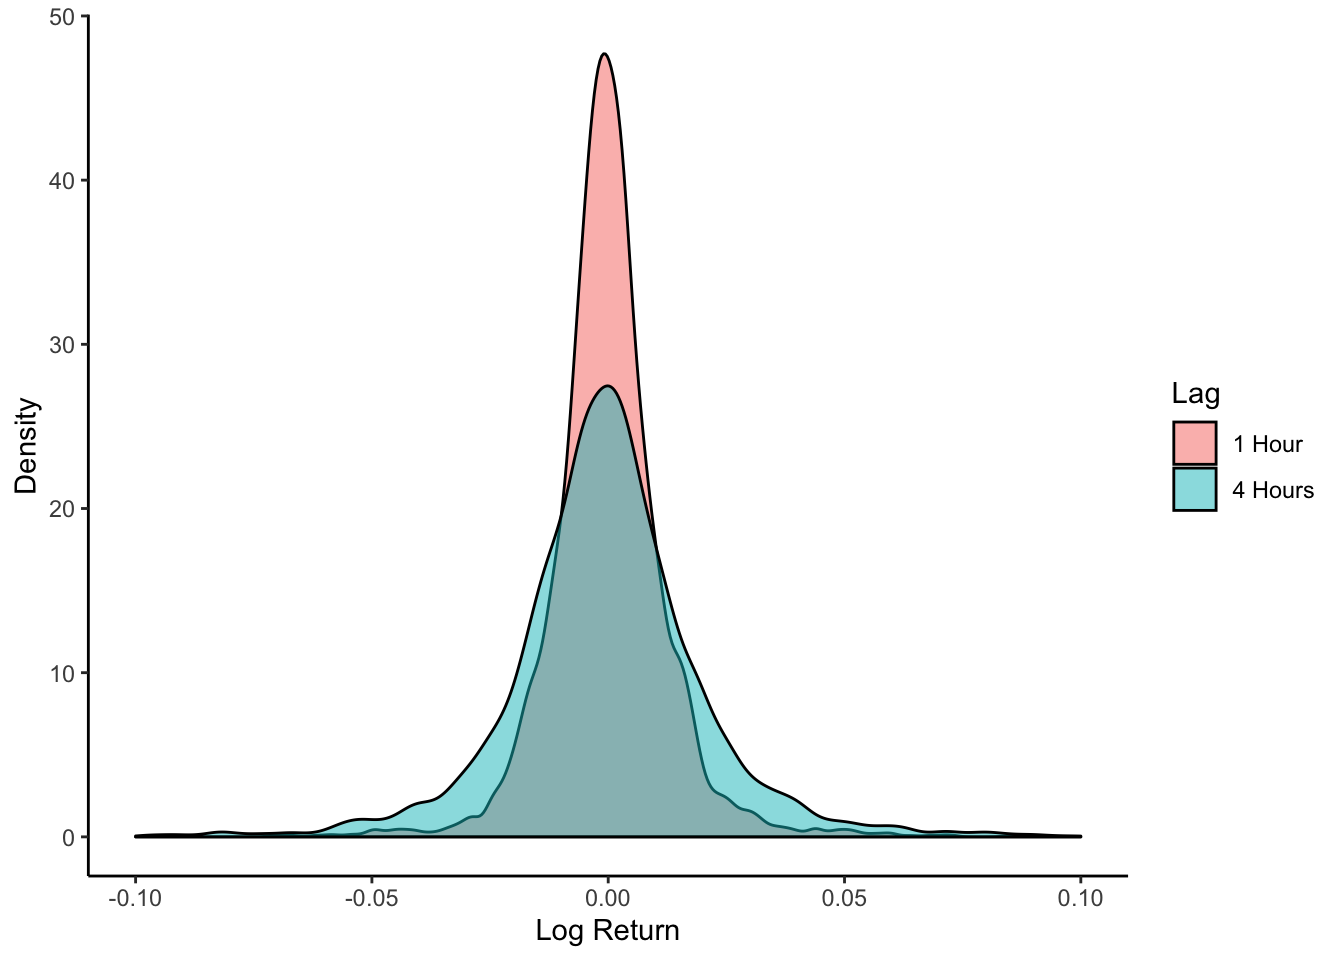
\includegraphics{thesis_files/figure-latex/logrets-1.pdf}
\caption{\label{fig:logrets}Distribution of Log Returns}
\end{figure}
\section{XGBoost}\label{xgboost}

Extreme Gradient Boosted Trees, XGBoost, is a decision tree based
ensemble learning method that employs boosting to efficiently yield high
accuracy predictions. Tree ensemble methods aggregate the predictions of
weak decision trees constantly updating residuals to improve
predictions. Assuming K regression trees, our prediction for point
\(y_i\) is the sum of the feature set \(\textbf{x}_i\) regressed on each
individual tree \(f_k\).
\begin{align}
  \hat{y_i} = \phi(\textbf{x}_i) = \sum_{k=1}^{K} f_k(\textbf{x}_i), \; \; f_k \in F \label{eq:1} \\ 
\end{align}
We minimize the following objective function where \(\Omega\) is a
regularization term that penalizes more complex models. \(T\) is the
number of leaves and w is the coefficient at each node. In my model
\(l\) is taken to be the mean squared error.
\begin{align}
  L(\phi) &= \sum_{i}^{} l(\hat{y}_i, y_i) + \sum_{k}^{} \Omega(f_k) \label{eq:2} \\ 
  \Omega(f) &= \gamma T +1/2 \lambda \| w \|\label{eq:3} \\ 
\end{align}
The model is trained in an iterative manner. If we let \(\hat{y}_i^(t)\)
be the prediction for point \(y_i\) at the \(t\) iteration than we
design \(f_t\) to minimize the following function.
\begin{align}
  L(\phi) = \sum_{i}^{n} [l(\hat{y}_i^{(t-1)}) + f_t(\textbf{x}_i), y_i)] + \Omega(f_t) \label{eq:4} \\ 
\end{align}
To achieve this I employ the following algorithm designed by Chen and
Guestrin (2016).
\begin{figure}
\centering
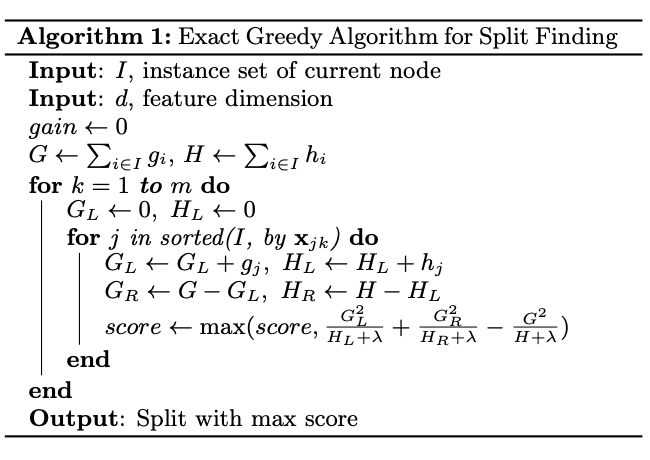
\includegraphics{figure/xgboost_algorithm.png}
\caption{}
\end{figure}
\section{Long Short-Term Memory}\label{long-short-term-memory}

Long Short-Term Memory is a type of recurrent neural network that due to
the specific architecture is able to better discern longer term
patterns, avoiding the vanishing gradient problem(Hochreiter \&
Schmidhuber, 1997). It has been used in many contexts, making notable
gains in speech recognition, language translation, and general time
series prediction(Beaufays, 2015).

The basic architecture of a memory cell in an LSTM network consists of
an input gate, forget gate, cell state, and output gate. The input gate
\(I_t\), forget gate \(F_t\), and output gate \(O_t\) for memory cell
\(t\) are linear combinations of the previous hidden state \(H_{t-1}\)
and current input \(X_t\) passed through the sigmoid function. I denote
the weight vectors as \(U\) and \(W\) and \(\odot\) and \(+\) denote
elementwise multiplication and addition.
\begin{align}
  I_t &= \sigma(X_t\odot W_i + H_{t-1}\odot U_i) \label{eq:6} \\ 
  F_t &= \sigma(X_t\odot W_f + H_{t-1}\odot U_f) \label{eq:7} \\ 
  O_t &= \sigma(X_t\odot W_o + H_{t-1}\odot U_o) \label{eq:8} \\ 
\end{align}
The cell state \(C_t\) is then a combination of the previous cell state
filtered by the forget gate and the input gate, which determines the
values to be updated, elementwise multiplied by another linear
combination of the hidden state and current input scaled by the tanh
function(Sanjeevi, 2018).
\begin{align}
  c_t &= \tanh(X_t\odot W_c + H_{t-1}\odot U_c) \label{eq:9} \\ 
  C_t &= \sigma(C_{t-1}\odot F_t + I_t\odot c_t) \label{eq:10} \\ 
\end{align}
The hidden state is the current state scaled by the tanh function
weighted by the output gate.
\begin{align}
  H_t = \tanh(C_t)\odot O_t \label{eq:11} \\ 
\end{align}
\subsection{Layers}\label{layers}

One challenge is determining the optimal number of hidden neurons and
hidden layers to avoid overfitting while still capturing potentially
complex interactions. From Jeff Heaton, one hidden layer can
``approximate any function that contains a continuous mapping from one
finite space to another''(2008). While I also tested using bidirectional
layers and multiple hidden layers, I achieved the greatest accuracy
through a single hidden layer.

\subsection{Dropout}\label{dropout}

Dropout is a common technique to reduce overfitting and make individual
hidden neurons more robust. Dropout refers to the random dropping of
individual neurons in the training phase. In an LSTM network, this can
take many different forms. After testing, I determined a 20 percent
recurrent dropout in the LSTM layer combined with a 40 percent dropout
layer was the most effective. Recurrent dropout in the context of LSTM
refers to dropping \(d\) during the update of the current state(G,
2018).
\begin{align}
  C_t &= \sigma(C_{t-1}\odot F_t + I_t\odot d(c_t)) \label{eq:12} \\ 
\end{align}
I then added the additional, stronger dropout layer on top of the LSTM
layer. I thus avoided a common issue in LSTM dropout in which important
past information is dropped, reducing the ability of the model to
identify long term patterns.

\subsection{Preprocessing}\label{preprocessing}

Unlike tree based models which are insensitive to the range of data,
LSTM perform best when the data is normalized. I normalized each feature
with the minimum and maximum of the training data\footnote{This avoids
  potential bias if the test data impacts the scaling}.

In addition, I used a sliding window lookback as seen in (Wei, 2018). I
found through validation that a lookback of 4 hours combined with 8
hidden units had the most success.

\chapter{Results}\label{results}

The hyperparameters for the models were tuned based on cross validation
performed on the first 30 percent of the timeseries (1,060 data points)
as shown in Figure \ref{fig:testing}. It should be noted that the test
period was a particularly volatile interval for Zcash, which doubled
before crashing back to below initial levels.
\begin{figure}
\centering
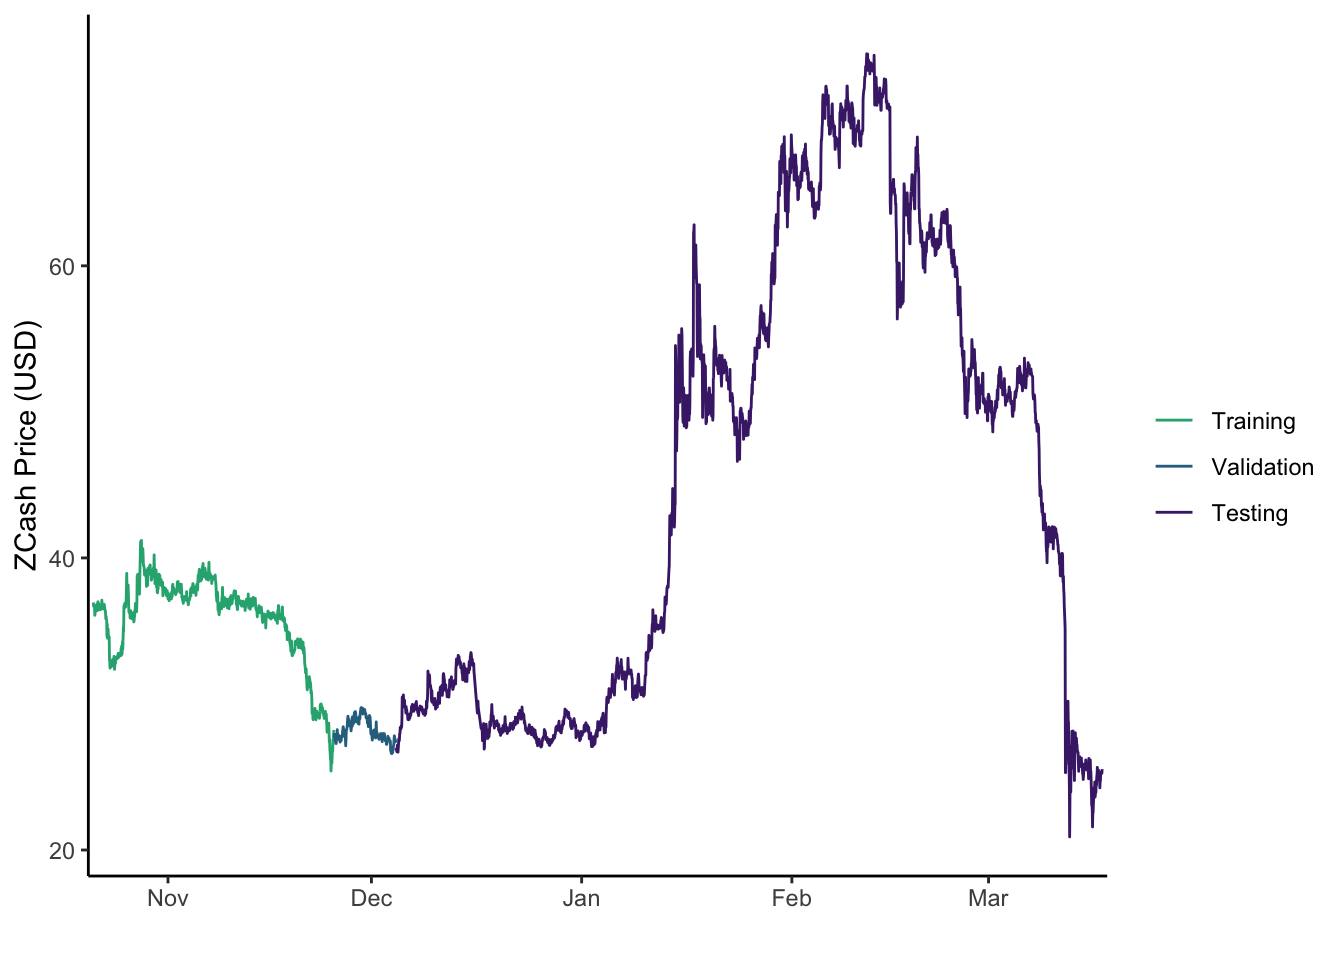
\includegraphics{thesis_files/figure-latex/testing-1.pdf}
\caption{\label{fig:testing}Zcash Price Across Training, Validation and
Testing Sets}
\end{figure}
Performance was measured using anchored\footnote{Unanchored walk-forward
  testing uses a sliding window of training data to remove outdated
  datapoints. This is unnecessary given the scope of training data.}
walk-forward testing, as seen in (Żbikowski, 2014), in which one
iteratively predicts test data point \(i\) using a model trained on data
points \((1:i-1)\)\footnote{As the model fits on four hour lagged
  returns, points \((i-4:i-1)\) will be correlated with point \(i\);
  therefore, this process was modified to train on points \((1:i-5)\).}.
This avoids the issue of look-ahead bias that occurs when standard cross
validation techniques are used on time series data, and allows us to
best simulate a live trading algorithm. Walk-forward testing provides a
more realistic measure of model performance as the model constantly
updates to include new market conditions and tests the stability of the
model to new data.

It should be noted that while the XGBoost model was retrained on the
insertion of each new data point, due to time constraints and to reduce
overfitting, the LSTM model was trained for one epoch every 50 new data
points, approximately two days of data. Both models were trained to
minimize root mean squared error.

\section{Trading Strategies}\label{trading-strategies}

The following strategies described in Table \ref{tab:strats} were tested
for both XGBoost and LSTM predictions, using the returns of holding
Zcash as a baseline strategy. One advantage of using prediction
percentiles instead of raw values to inform strategies is that it
improves the balance between the number of buy/sell trades, reducing the
impact of directional bias. I tested both an exponential decay and
weighting by prediction value, however these approaches did not yield
significantly better results. The percentiles of predictions were
calculated for prediction \(i\) on the set of predictions \((1:i)\) with
the notable exception being that the first ten percent of test data
points were grouped together.

\label{tab:strats}Strategy Descriptions

Strategies

Descriptions

Hold

Return of holding Zcash

All

Trade on every increment, direction in comparison to mean prediction

Top 20

Trade on the top and bottom 20 percent of predictions

Top 10

Trade on the top and bottom 10 percent of predictions

The predictions for the XGBoost and LSTM models are displayed below in
Figures \ref{fig:xgboostTrades} and \ref{fig:lstmTrades}. The points are
subsetted based on the Top 20 trading strategy. The XGBoost predictions
are more evenly distributed throughout the time series, whereas the LSTM
predictions follow clear trends.
\begin{figure}
\centering
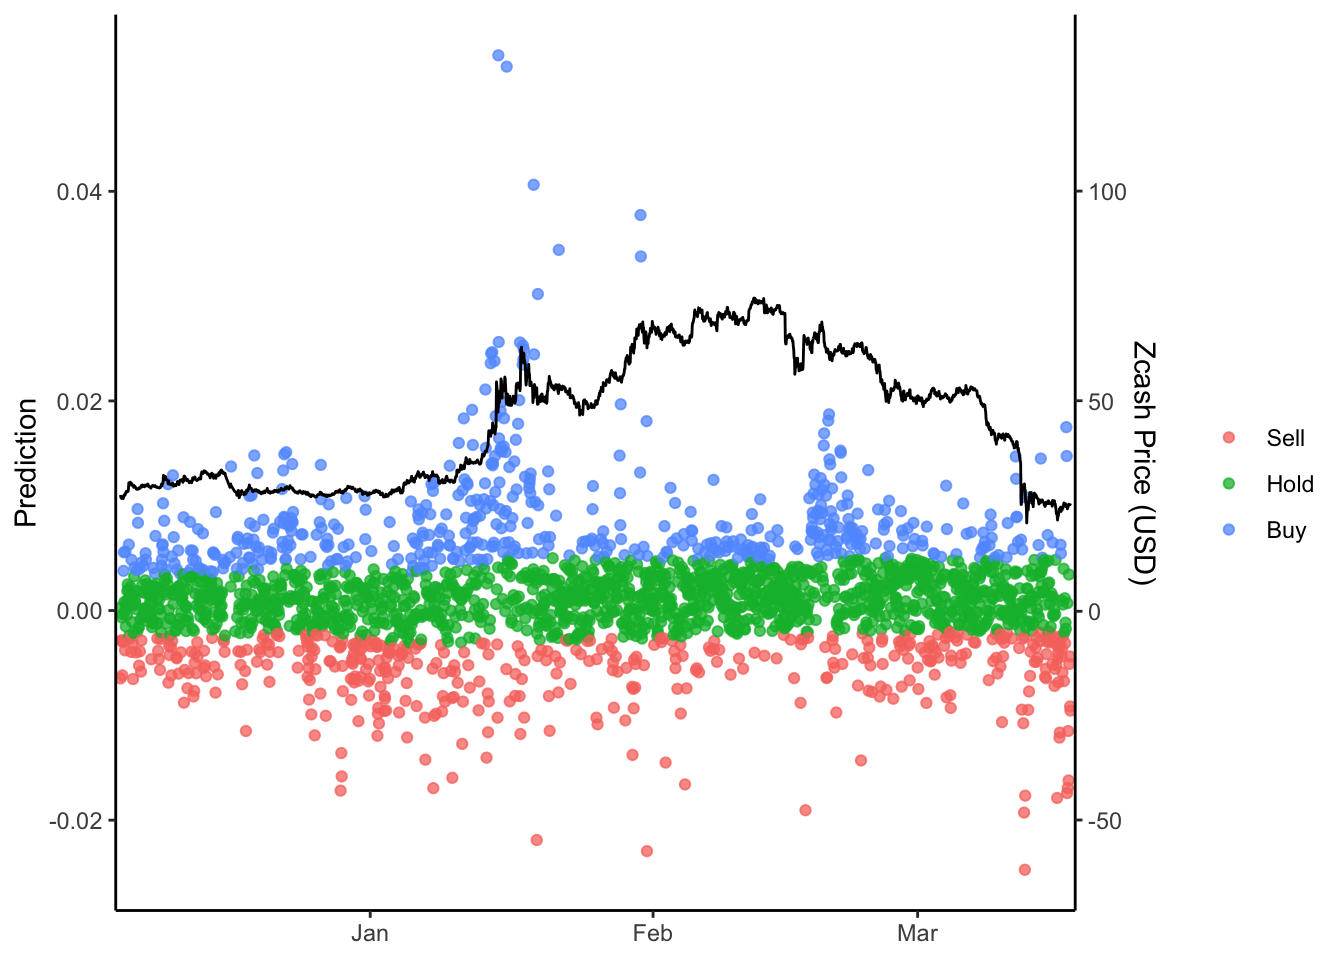
\includegraphics{thesis_files/figure-latex/xgboostTrades-1.pdf}
\caption{\label{fig:xgboostTrades}XGBoost Predictions}
\end{figure}
\begin{figure}
\centering
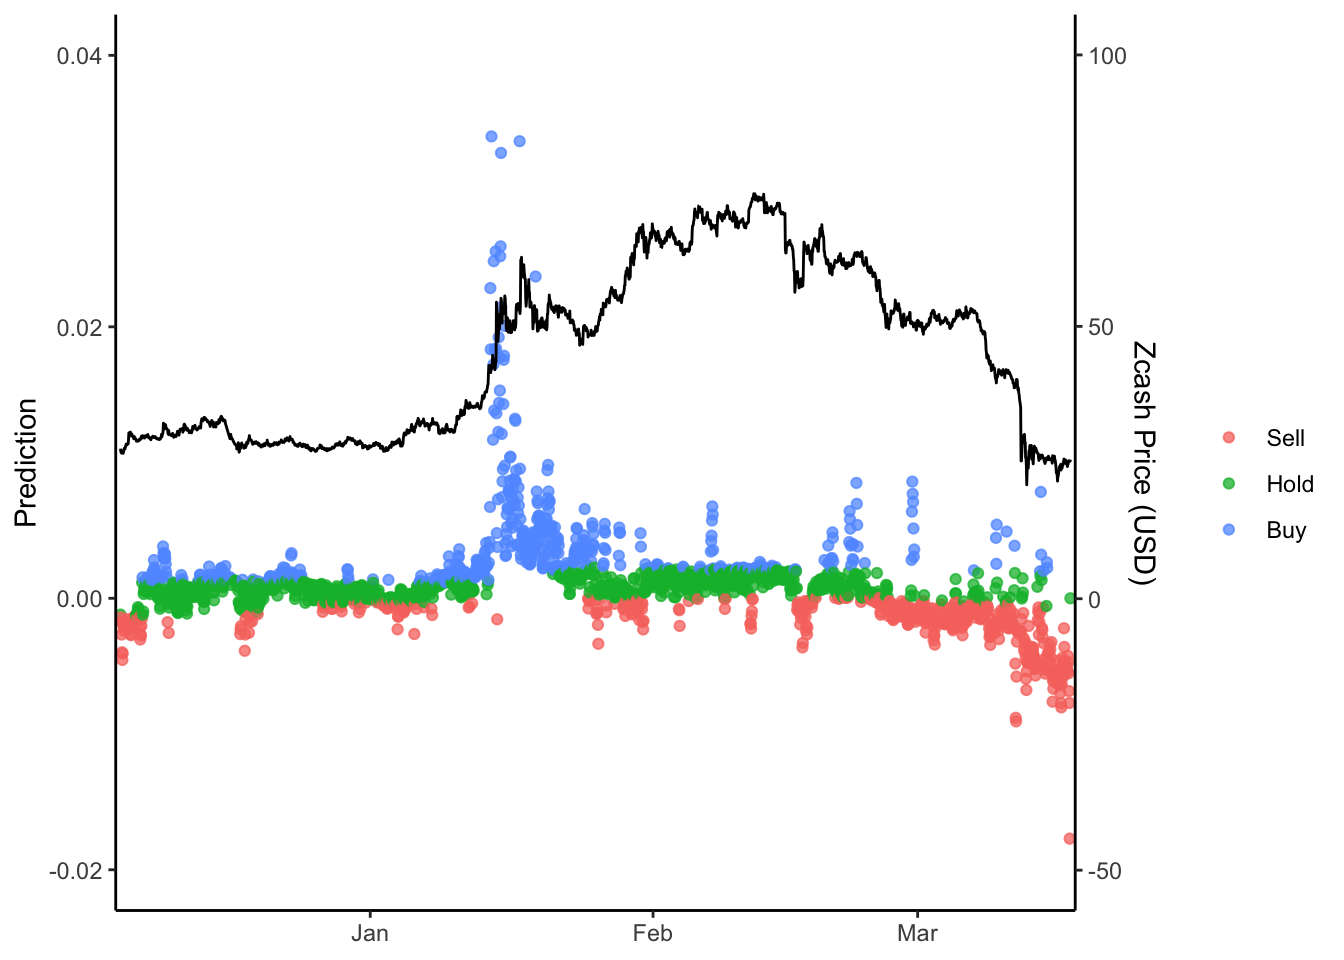
\includegraphics{thesis_files/figure-latex/lstmTrades-1.pdf}
\caption{\label{fig:lstmTrades}LSTM Predictions}
\end{figure}
\section{Performance}\label{performance}

While the models achieved the best performance when trained on 4 hour
log returns, we actually see that the performance accumulates past 4
hours. We see a monotonic increase in mean performance across all the
strategies in Figure \ref{fig:pnltime} up to 5 hours after the trade.
The LSTM and XGBoost Top 20 strategies return over a third of a percent
per trade.
\begin{figure}
\centering
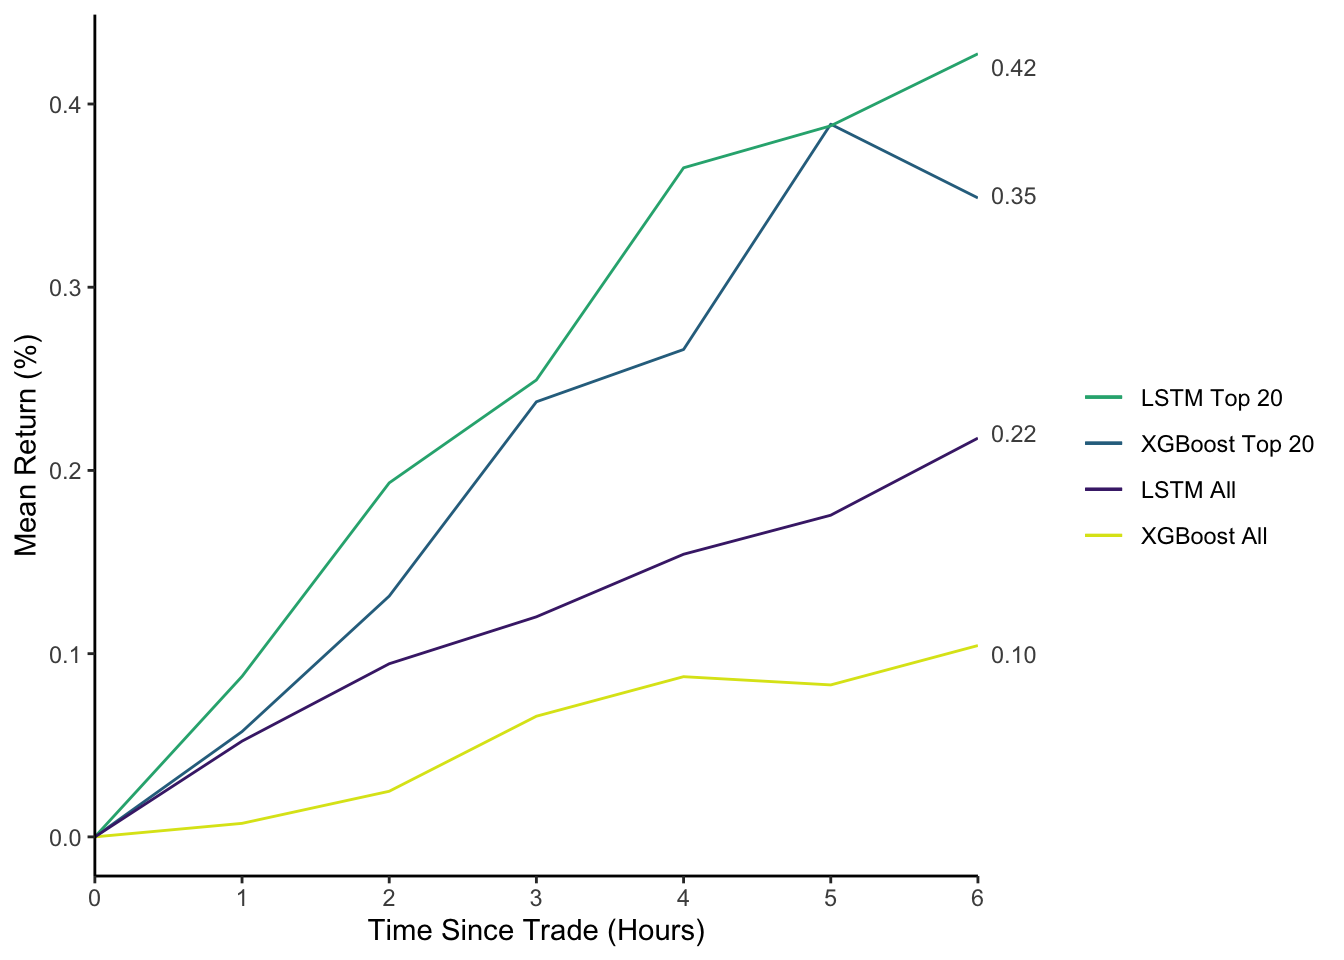
\includegraphics{thesis_files/figure-latex/pnltime-1.pdf}
\caption{\label{fig:pnltime}Per Trade PNL}
\end{figure}
Per trade returns are slightly misleading as many signals overlap,
resulting in actual profits that are much lower than pure sum of mean
returns. Figures \ref{fig:xgboostPnls} and \ref{fig:LSTMPnls} display
the theoretical returns of the strategies over the testing period. In
the implementation of these strategies it is assumed that new signals
override old predictions and after 5 hours of no prediction the position
is closed.
\begin{figure}
\centering
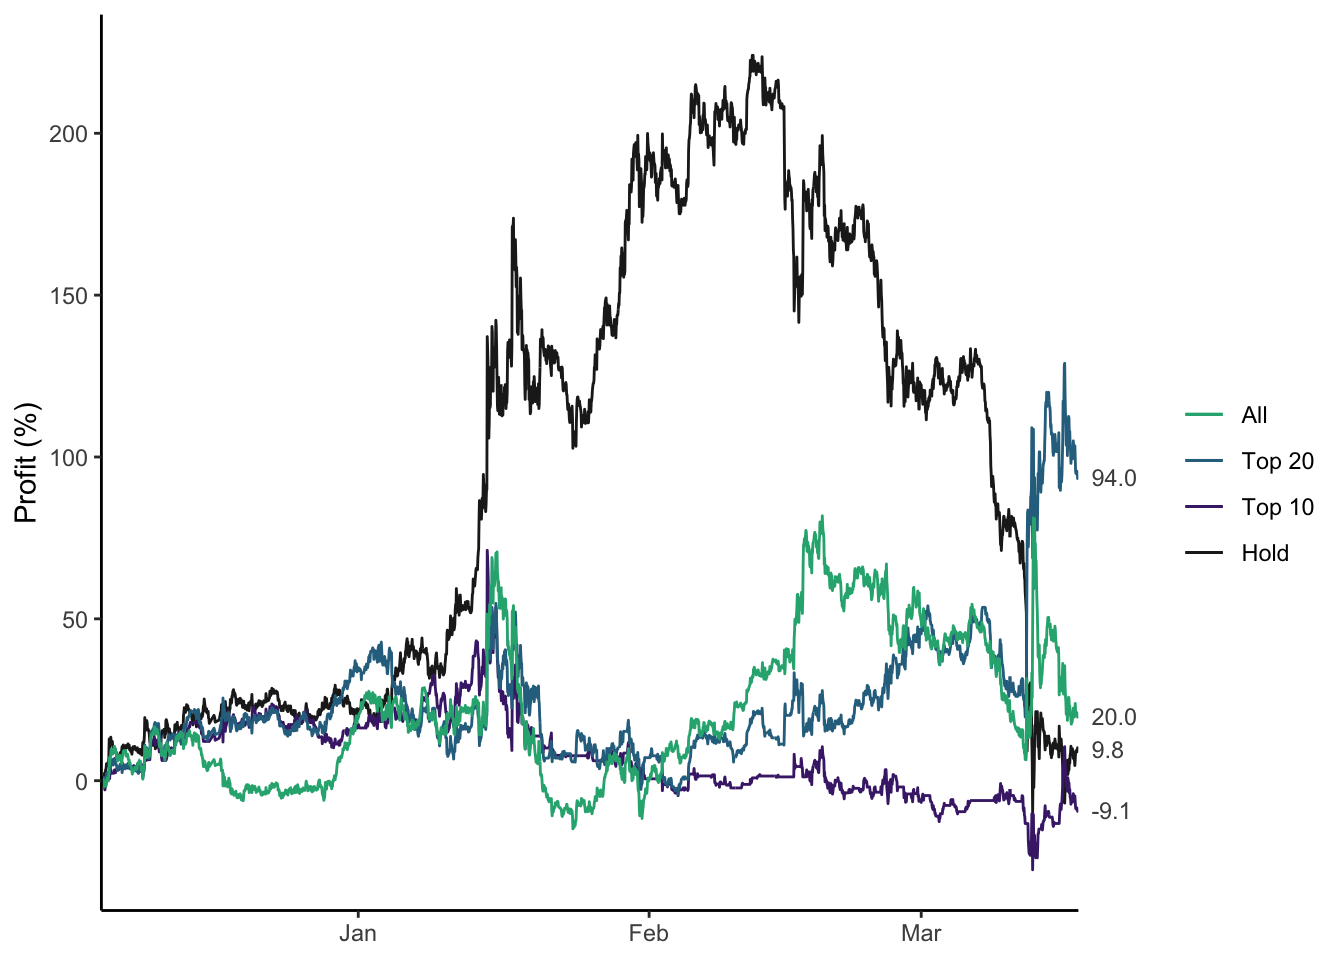
\includegraphics{thesis_files/figure-latex/xgboostPnls-1.pdf}
\caption{\label{fig:xgboostPnls}XGBoost Strategies PNL}
\end{figure}
\begin{figure}
\centering
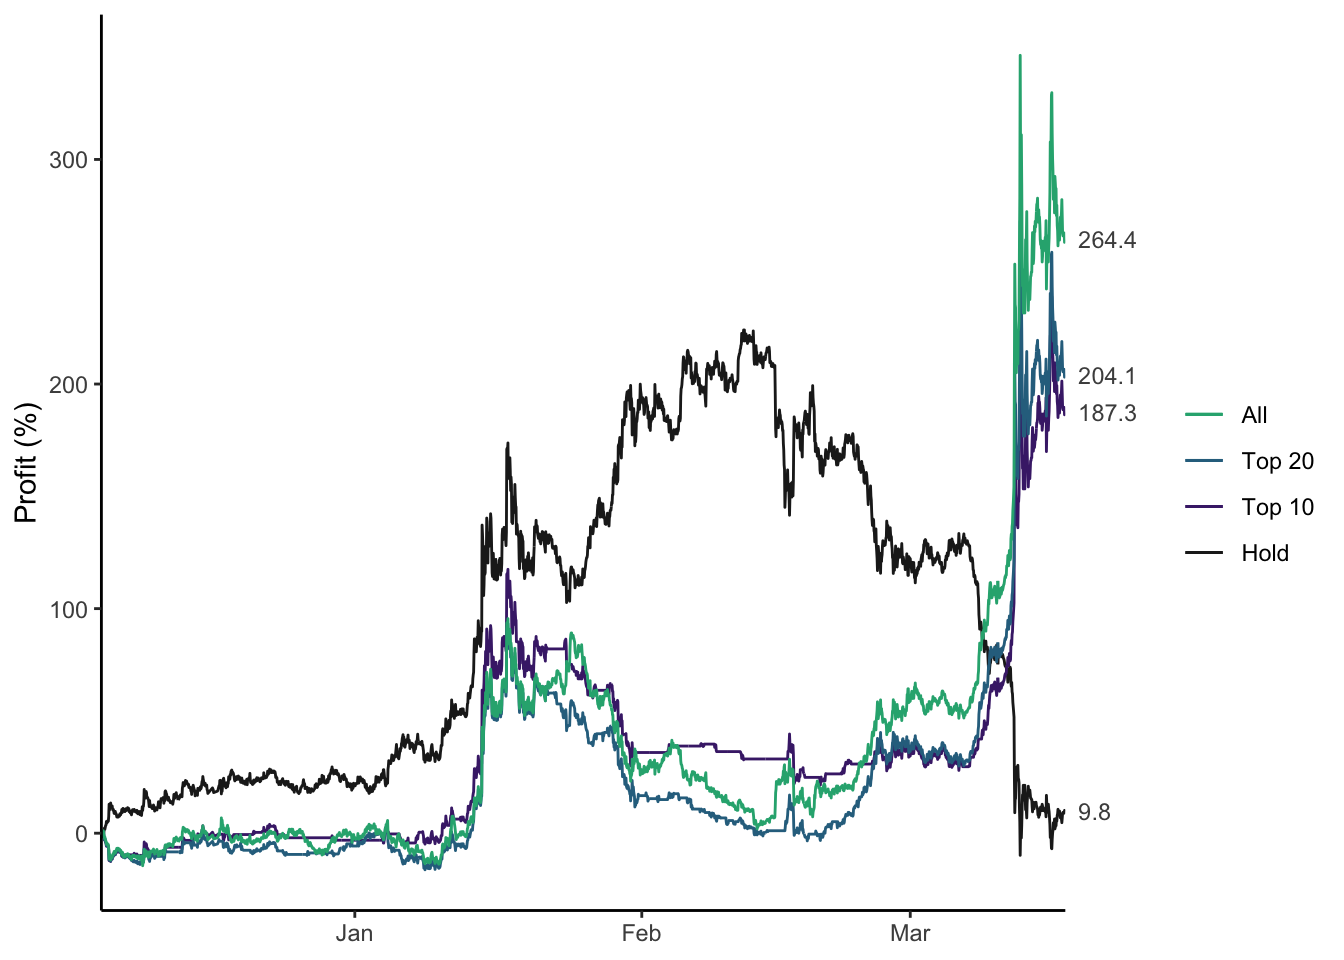
\includegraphics{thesis_files/figure-latex/LSTMPnls-1.pdf}
\caption{\label{fig:LSTMPnls}LSTM Strategies PNL}
\end{figure}
All three LSTM strategies outperform the most profitable XGBoost
strategy. The LSTM All and Top 20 strategies both return over 200
percent in just over 100 days while the XGBoost Top 20 strategy also
produces sizeable returns of 94 percent. Every strategy except the
XGBoost Top 10 outperforms the market during this time period.

While by no means a perfect metric, the Sharpe ratio is a strong proxy
for risk adjusted returns. It is the excess expected return compared to
the risk free rate \(R_f\) divided by the standard deviation of returns.
\begin{align}
  Sharpe = \frac{E(Return - R_f)}{sd(Return - R_f)}\label{eq:1} \\ 
\end{align}
Using a risk free rate of 2\%, Table \ref{tab:sharpe} displays the
Sharpe ratio for the following strategies. This is calculated with daily
returns, and then scaled by the square root of days in a calendar year.

\label{tab:sharpe}Sharpe Ratios

XGBoost Top 20

LSTM Top 20

LSTM All

Sharpe Ratio

3.11

2.67

2.67

While these strategies display strong Sharpe ratios, they are depressed
by the large volatility in the test data. Although the XGBoost 20
strategy was less profitable it has a higher Sharpe ratio becuase of
less volatility in its returns.

\section{Performance Net Fees}\label{performance-net-fees}

Transaction costs represent a considerable expense in the cryptocurrency
market. As a point of reference, Binance, one of the largest
cryptocurrency exchanges, charges transaction fees of between 1.5 to 7.5
basis points\footnote{One hundredth of one percent}. While spreads are
generally fairly negligible on liquid markets, during times of high
volatility they can represent an additional 5-10 basis points. Table
\ref{tab:feetable} displays the strategy profits assuming different fee
structures. It is clear that even with substantial transaction fees
these strategies remain profitable. However, when taking transaction
fees into account it would be advantageous to only trade on the most
profitable subset of signals.

\label{tab:feetable}Percent Returns Net Fees

15 bps

5 bps

2.5 bps

XGBoost Top 20

11.5\%

61.3\%

76.9\%

LSTM Top 20

156.7\%

187.4\%

195.7\%

LSTM All

134.7\%

214.7\%

238.6\%

\chapter*{Discussion}\label{discussion}
\addcontentsline{toc}{chapter}{Discussion}

\section{Limitations}\label{limitations}

Though this model displays a notable edge in testing, it is important to
recognize potential limitations that might make it unprofitable in
practice.

To begin, there may be a mismatch between the prices in my dataset and
the price point of actionable liquidity. As some of these exchanges
operate in only a subset of countries, it may be the case that I have a
theoretical edge, but in practice the trades would not be possible at
the price points displayed. This might be the case if aggregated price
points oscillate in weightings between different exchanges.

Secondly, my edge may be real but simply not account for black swan
events. While I may have an on average profitable strategy, the risk
adjusted rate of returns are poor.

Lastly, there is the possibility that these returns are due to pure
chance. While this is a large dataset and we see strong average returns,
a few small timeframes account for most of the price movement. These
profits could be attributable to a few correct predictions or a few
associations that only by accident work in this context. Back testing is
a tedious process in which many false associations may be found.

\section{Conclusion}\label{conclusion}

The goal of this thesis is to demonstrate strategies that produce
substantial alpha in an altcoin market. While I am cognizant of
potential limitations, it seems likely that these strategies capture
legitimate alpha by parsing out signal from a combination of features.
Other studies have shown similar predictive power in Bitcoin and here I
add proof of concept that models using both sentiment and volume based
indicators can be similarly accurate in a smaller market with a fraction
of the data.

\section{Future Work}\label{future-work}

Additional research can improve upon the sentiment and bot
classification algorithms used in this study. These algorithms can be
tuned specifically to the context of cryptocurrency to achieve more
accurate categorization. Furthermore, additional research should explore
hedging strategies that would help reduce the variance of returns,
therefore improving the risk adjusted returns.

\appendix


\chapter{Appendix A}\label{appendix-a}

\section{Model Features}\label{model-features}

Zcash Gtrend

Zcash Gtrend Ratio

ZEC Gtrend Ratio

Volume From

Volume To

Tweet Count

Mean Sentiment

Sentiment Retw. Weighted

33

1.100000

2.133333

461959.8

12541.98

12

0.0573850

0.0000053

46

1.586207

1.551724

516757.6

14040.55

7

0.1481721

0.0833144

40

1.481481

2.296296

910020.4

24811.14

9

0.0196764

0.0000000

35

1.206897

2.620690

943465.4

25714.64

5

0.0097706

0.0908355

26

0.962963

2.518518

879135.5

24370.13

14

0.0735963

0.1326699

\section{QQ Plot of Log Returns}\label{qq-plot-of-log-returns}
\begin{figure}
\centering
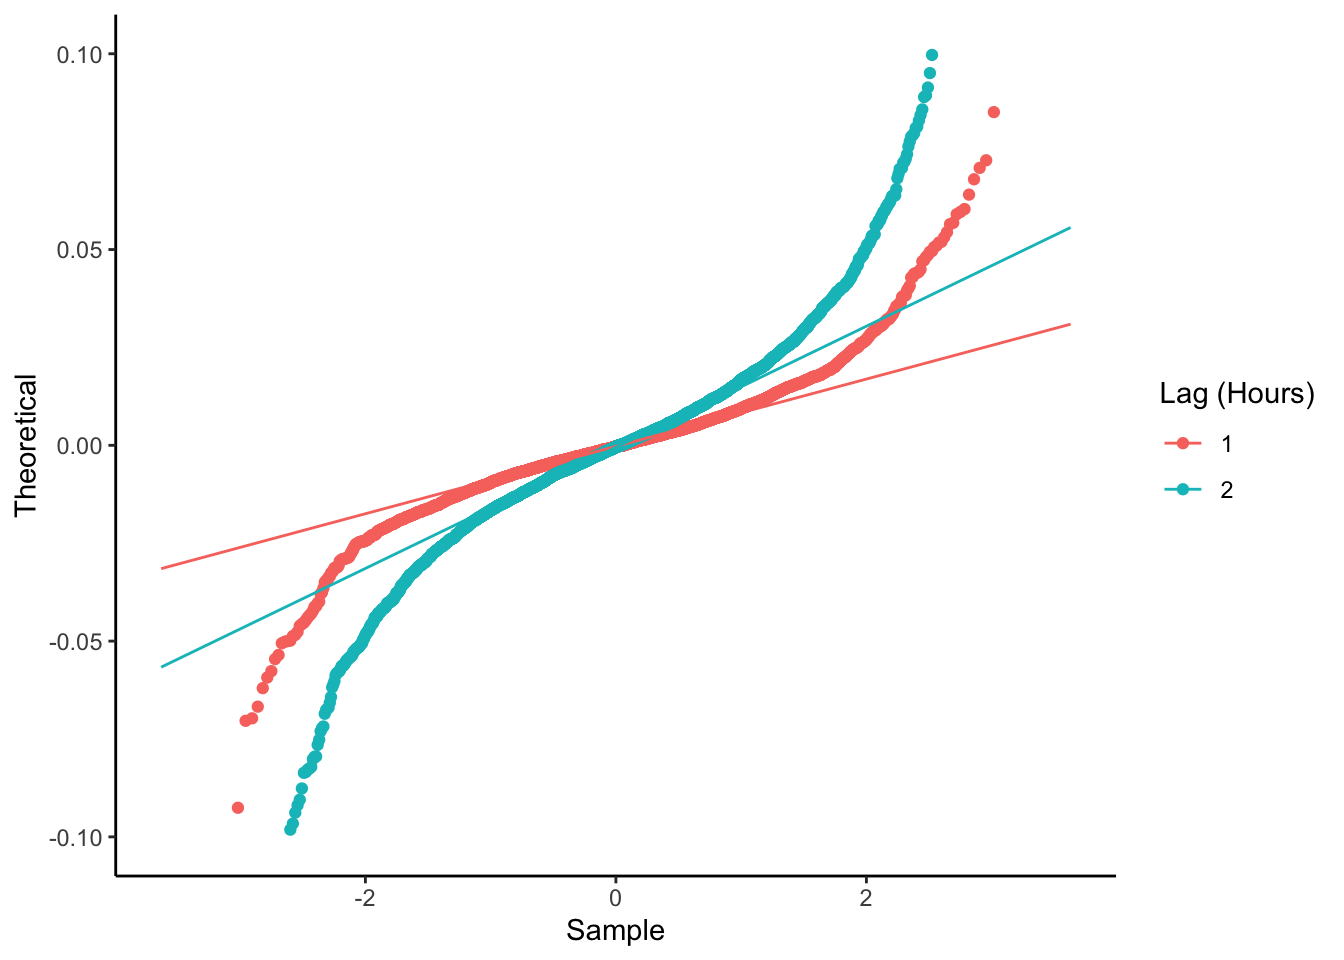
\includegraphics{thesis_files/figure-latex/unnamed-chunk-9-1.pdf}
\caption{}
\end{figure}
\section{Returns Net Fees}\label{returns-net-fees}
\begin{figure}
\centering
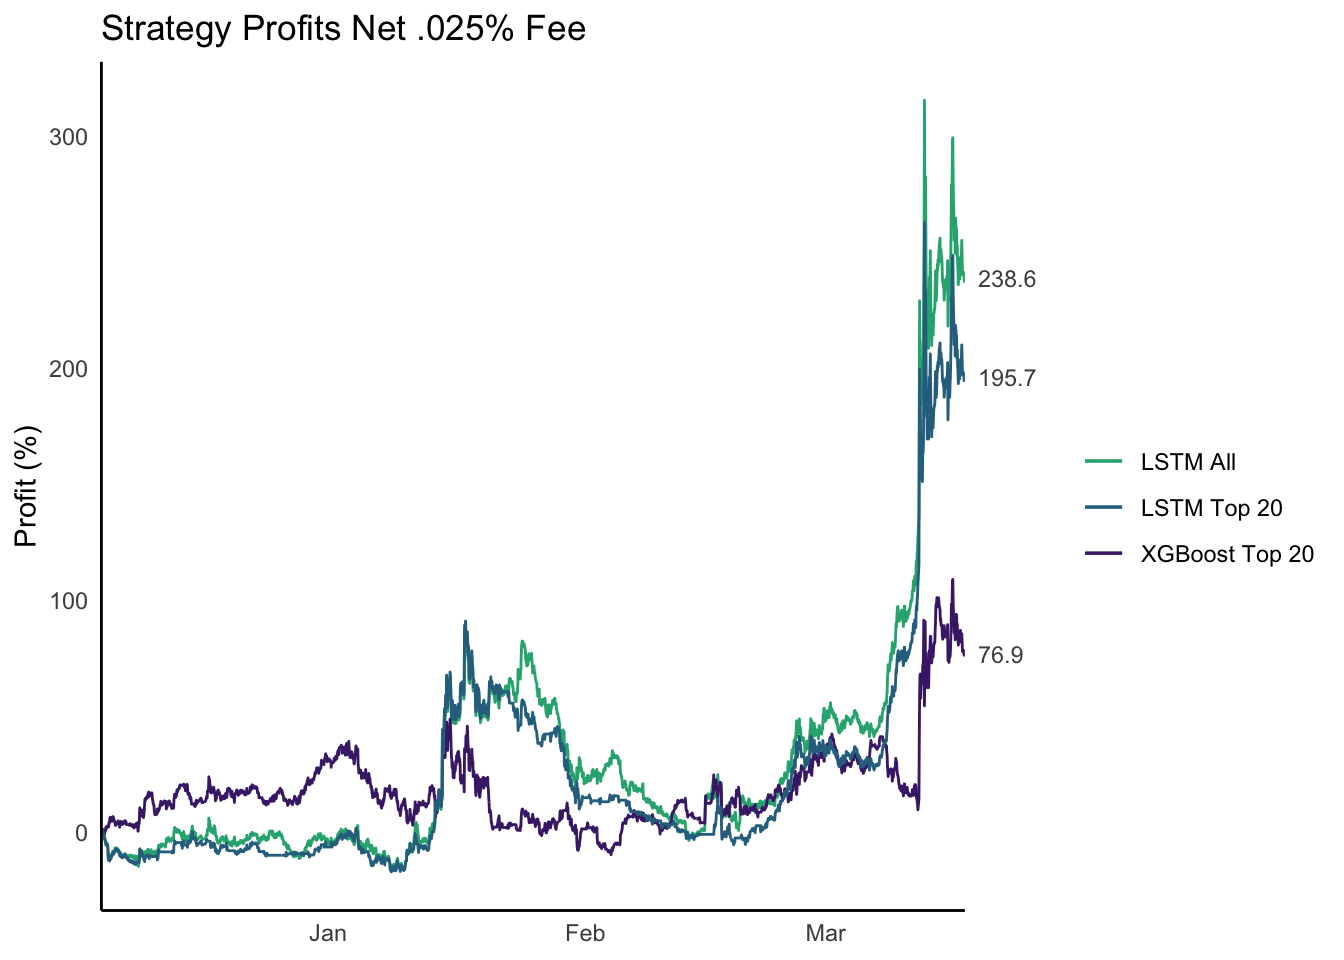
\includegraphics{thesis_files/figure-latex/unnamed-chunk-10-1.pdf}
\caption{}
\end{figure}
\backmatter

\chapter*{References}\label{references}
\addcontentsline{toc}{chapter}{References}

\markboth{References}{References}

\noindent

\setlength{\parindent}{-0.20in} \setlength{\leftskip}{0.20in}
\setlength{\parskip}{8pt}

\hypertarget{refs}{}
\hypertarget{ref-beaufays2015}{}
Beaufays, F. (2015, August). Google ai blog. \emph{Google AI Blog}.
Retrieved from
\url{ai.googleblog.com/2015/08/the-neural-networks-behind-google-voice.html}

\hypertarget{ref-chen2016}{}
Chen, T., \& Guestrin, C. (2016). Xgboost: A scalable tree boosting
system. In \emph{Proceedings of the 22nd acm sigkdd international
conference on knowledge discovery and data mining} (pp. 785--794).

\hypertarget{ref-colianni2015}{}
Colianni, S., Rosales, S., \& Signorotti, M. (2015). Algorithmic trading
of cryptocurrency based on twitter sentiment analysis.

\hypertarget{ref-dickerson2018}{}
Dickerson, A. (2018). Algorithmic trading of bitcoin using wikipedia and
google search volume. Retrieved from
\url{http://dx.doi.org/10.2139/ssrn.3177738}

\hypertarget{ref-elbahrawy2019}{}
ElBahrawy, A., Alessandretti, L., \& Baronchelli, A. (2019). Wikipedia
and cryptocurrencies: Interplay between collective attention and market
performance.

\hypertarget{ref-floyd2018}{}
Floyd, D. (2018). Zcash privacy weakened by certain behaviors,
researchers say. Retrieved from
\url{www.coindesk.com/zcash-privacy-weakened-by-certain-behaviors-researchers-say}

\hypertarget{ref-g2018}{}
G, A. (2018). A review of dropout as applied to rnns. medium.

\hypertarget{ref-garcia2015}{}
Garcia, D., \& Schweitzer, F. (2015). Social signals and algorithmic
trading of bitcoin. \emph{Society Open Science}, \emph{2}(9).

\hypertarget{ref-heaton2008}{}
Heaton, J. (2008). \emph{Introduction to neural networks for java, 2nd
edition} (2nd ed.). Heaton Research, Inc.

\hypertarget{ref-sepp1997}{}
Hochreiter, S., \& Schmidhuber, J. (1997). Long short-term memory.
\emph{Neural Computation}, \emph{9}(8), 1735--1780.
\url{http://doi.org/10.1162/neco.1997.9.8.1735}

\hypertarget{ref-kim2017}{}
Kim, Y., Lee, J., Park, N., Choo, J., Kim, J., \& al. (2001). When
bitcoin encounters information in an online forum: Using text mining to
analyse user opinions and predict value fluctuation. Retrieved from
\url{https://doi.org/10.1371/journal.pone.0177630}

\hypertarget{ref-koning2019}{}
Koning, J. (2019, November). Moneyness. \emph{Moneyness}.

\hypertarget{ref-kristoufek2013}{}
Kristoufek, L. (2013). BitCoin meets google trends and wikipedia:
Quantifying the relationship between phenomena of the internet era.
\emph{Scientific Reports}, \emph{3}(1).

\hypertarget{ref-li2019b}{}
Li, T., Chamrajnagar, A., Fong, X., Rizik, N., \& Fu, F. (2019).
Sentiment-based prediction of alternative cryptocurrency price
fluctuations using gradient boosting tree model. \emph{Front. Phys.}

\hypertarget{ref-li2019a}{}
Li, T., Shin, D., \& Wang, B. (2019). Cryptocurrency pump-and-dump
schemes. Retrieved from \url{http://dx.doi.org/10.2139/ssrn.3267041}

\hypertarget{ref-mills2019}{}
Mills, D. J., \& Nower, L. (2019). Preliminary findings on
cryptocurrency trading among regular gamblers: A new risk for problem
gambling? \emph{Addictive Behaviors}, \emph{92}, 136--140.

\hypertarget{ref-oliviera2017}{}
Oliveira, N., Corteza, P., \& Areal, N. (2017). Analyzing stock market
movements using twitter sentiment analysis. Retrieved from
\url{http://repositorium.sdum.uminho.pt/bitstream/1822/54457/4/paper.pdf}

\hypertarget{ref-sanjeevi2018}{}
Sanjeevi, M. (2018, January). Chapter 10.1: DeepNLP --- lstm (long short
term memory) networks with math.

\hypertarget{ref-rao2012}{}
Tushar, R., \& Srivastava, S. (2012). Analyzing stock market movements
using twitter sentiment analysis. \emph{International Conference on
Advances in Social Networks Analysis and Mining}. Retrieved from
\url{http://dx.doi.org/10.1109/ASONAM.2012.30}

\hypertarget{ref-varol2017}{}
Varol, O., Ferrara, E., Davis, C. A., Menczer, F., \& Flammini, A.
(2017). Online human-bot interactions: Detection, estimation, and
characterization. In \emph{Eleventh international aaai conference on web
and social media}.

\hypertarget{ref-vernon2003}{}
Vernon, A. M. (2003). Market efficiency and march madness: Empirical
tests of point spread betting. \emph{SSRN Electronic Journal}.

\hypertarget{ref-wei2018}{}
Wei, J. (2018, December). Predicting cryptocurrency prices with machine
learning. Retrieved from
\url{medium.com/datadriveninvestor/predicting-cryptocurrency-prices-with-machine-learning-1b5a711d3937}

\hypertarget{ref-quant2012}{}
Why log returns. (2012, November). Quantivity. Retrieved from
\url{quantivity.wordpress.com/2011/02/21/why-log-returns.}

\hypertarget{ref-wojcik2018}{}
Wojcik, S. (n.d.). 5 things to know about bots on twitter. Retrieved
from
\url{https://www.pewresearch.org/fact-tank/2018/04/09/5-things-to-know-about-bots-on-twitter/}

\hypertarget{ref-zib2014}{}
Żbikowski, K. (2014). Using volume weighted support vector machines with
walk forward testing and feature selection for the purpose of creating
stock trading strategy. \emph{Expert Systems with Applications},
\emph{42}. \url{http://doi.org/10.1016/j.eswa.2014.10.001}


% Index?

\end{document}
